%!TEX root = ../../../adrien_gomar_phd.tex

The same topology and number of grid points is used to
mesh this high-speed configuration. 
If nothing particular is said, the same numerical parameters
are considered to be kept for the study of this
high-speed configuration.
The reader is referred to 
Sec.~\ref{sec:dream_ls_numerical} for detailed information.

The same numerical approach as the low-speed configuration
is chosen for the aeroelastic computations presented in
Sec.~\ref{sec:dream_hs_ael_results}.
For practical reasons, the harmonic balance computations are run with
only five frequencies in total. This might be not sufficient
as suggests the prediction tool shown in 
Sec.~\ref{sec:dream_hs_spectral_convergence}.
Nevertheless, in the rear rotor,
the harmonics of the front rotor blade passing frequency
are chosen. In the front rotor, the first frequency is the
frequency associated to the vibration of the blade and the
remaining ones are harmonics of the rear rotor blade 
passing frequency. 
The time instances are automatically chosen using the OPT
algorithm (see Sec.~\ref{sec:algo_opt}) which leads to 
a condition number always lower than $1.1$ which ensure
the convergence of the computations.


\paragraph{Influence of the number of harmonics for the aeroelastic simulations}
\label{sub:dream_hs_convergence_ael}

To assess the convergence of the capture of the damping by the multi-frequential
HB approach, four computations are run on the second flection mode
of the high-speed CROR configuration. For each computation, the 
vibration frequency is considered with one to several harmonics
of the blade passing frequency of the rear rotor. As indicated in
Sec.~\ref{par:choice_of_frequencies}, several approaches exist to
truncate the frequency sets. Here, only the "cross grid" truncation 
pattern is used with only one aeroelastic frequency.
\begin{figure}[htp]
 \ra{1.3} \centering
 \begin{tabular}{r|cccc}
   \toprule
   & \multicolumn{4}{c}{
        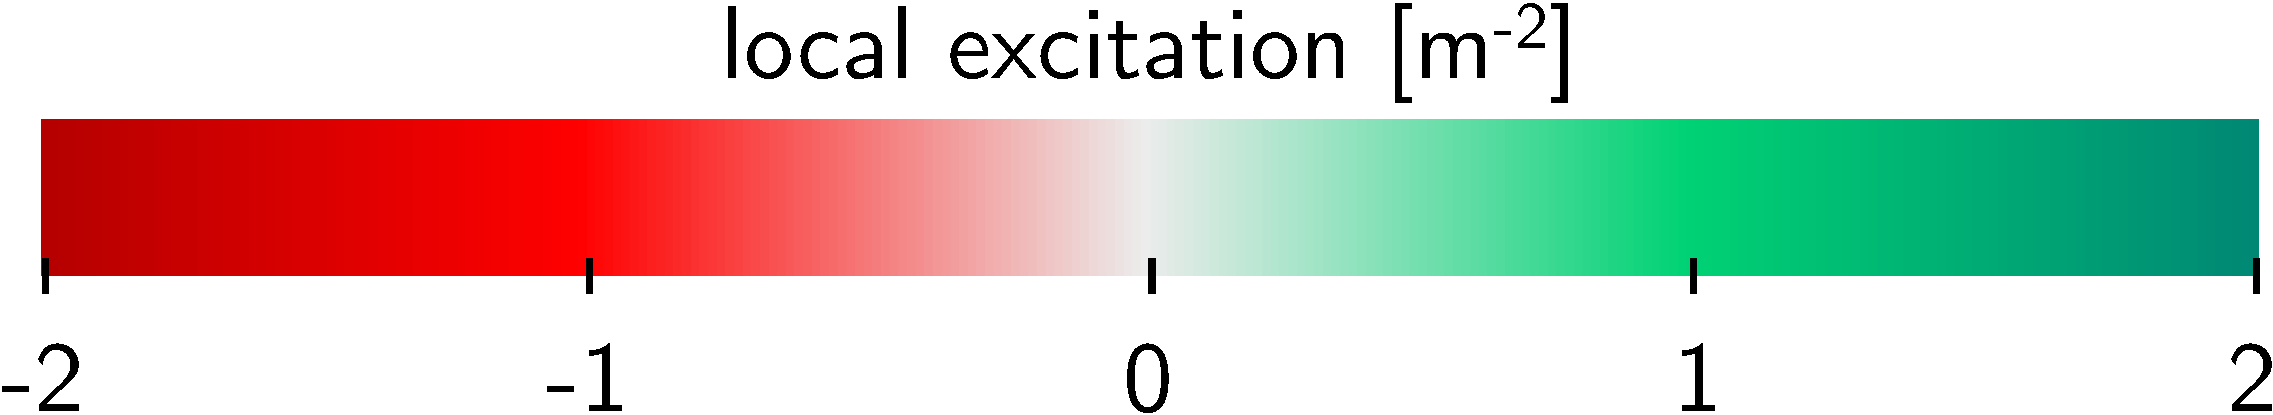
\includegraphics[width=0.22\textwidth]{dream_hs_damping_scale.pdf}} \\
   & $N=2$ & $N=3$ & $N=4$ & $N=5$ \\
   \midrule
   \rotatebox{90}{\quad\quad\quad suction side} 
   & 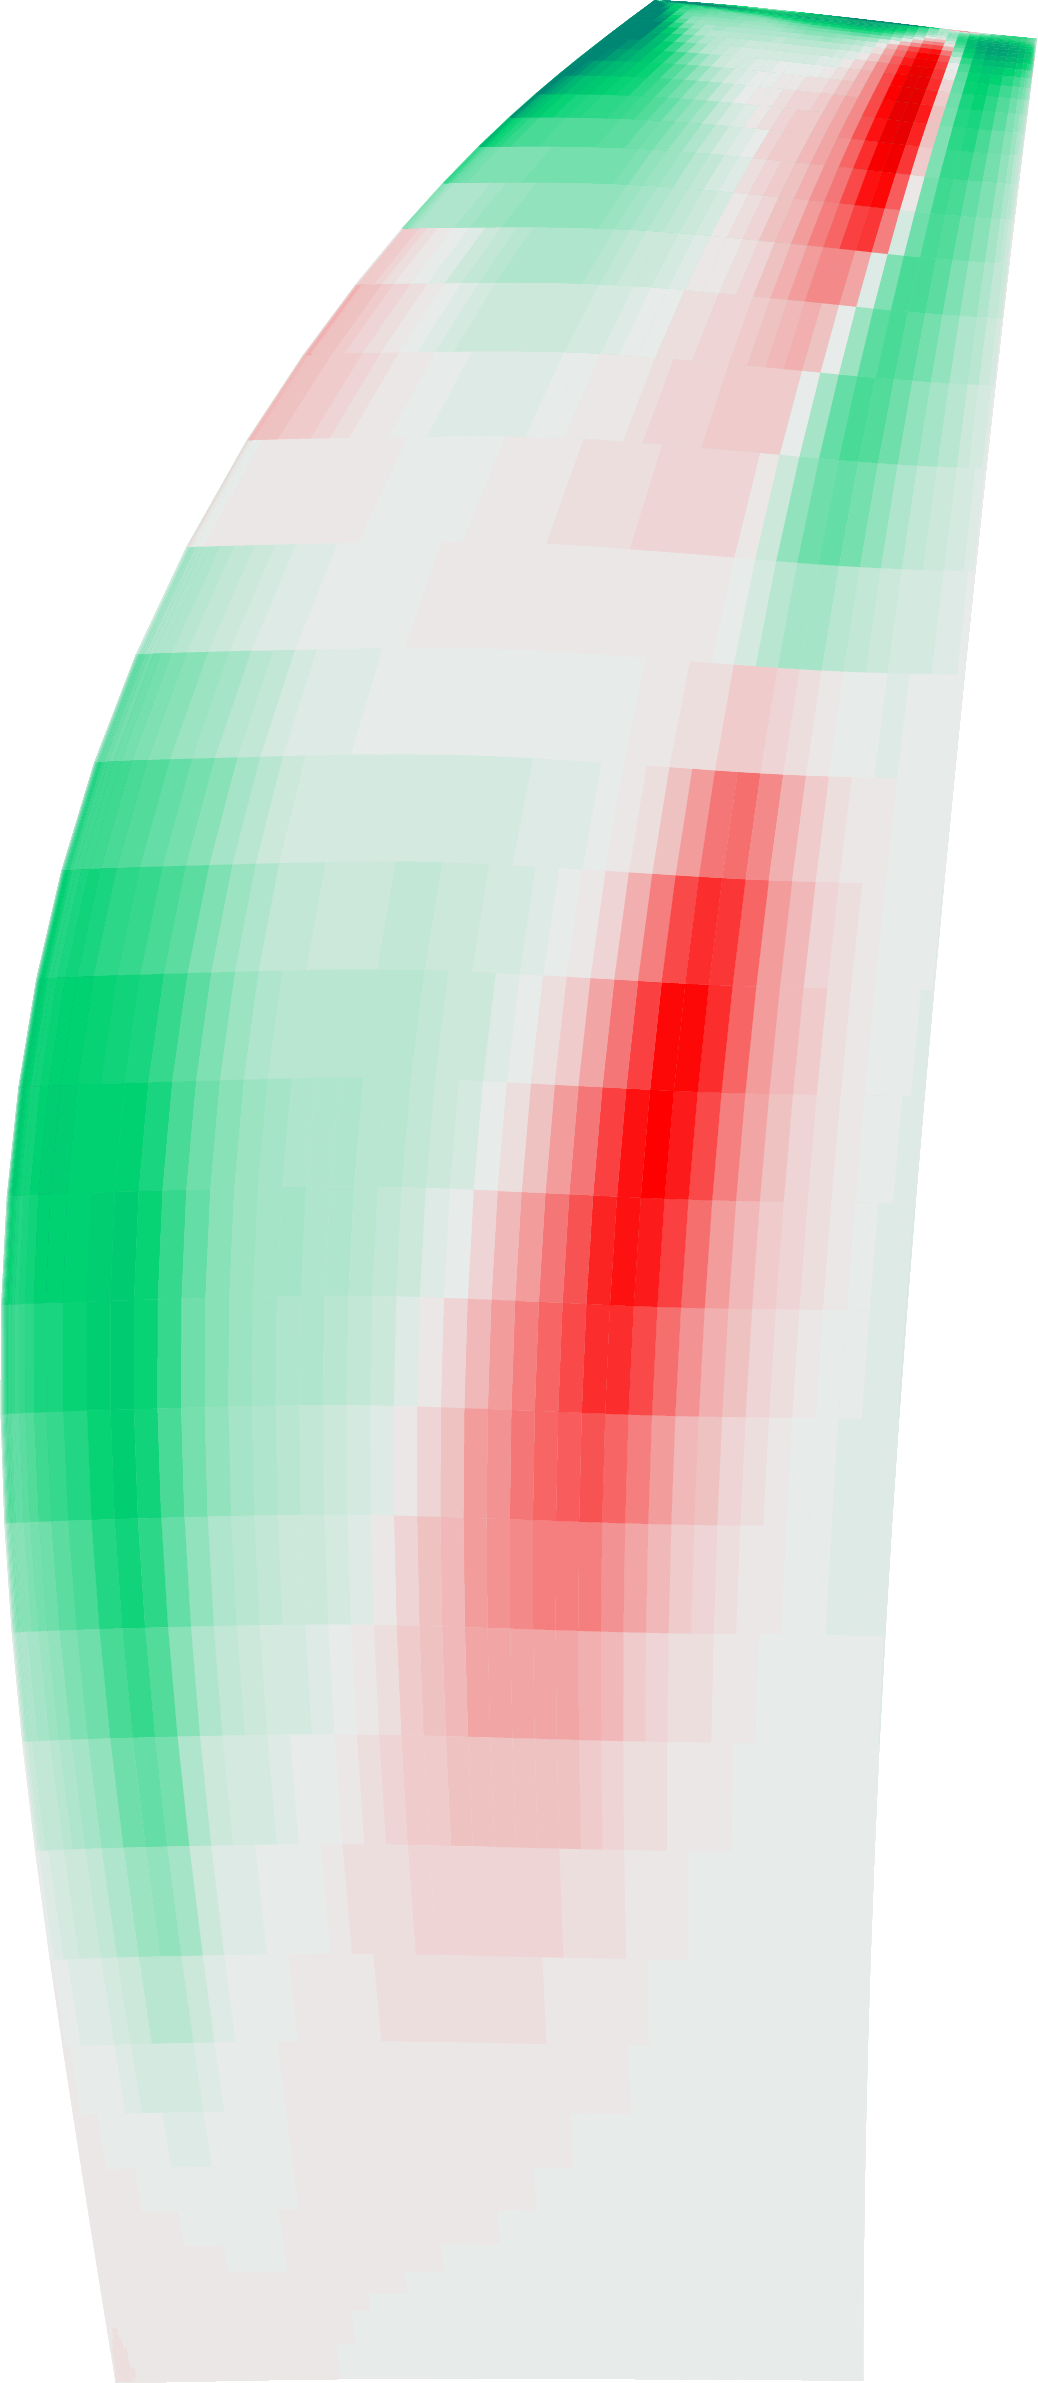
\includegraphics[width=0.12\textwidth]{DREAM_HS_HBT_N2_AEL_H1M2FD-1_roe3_sa_local_damping_SS.png}
   & 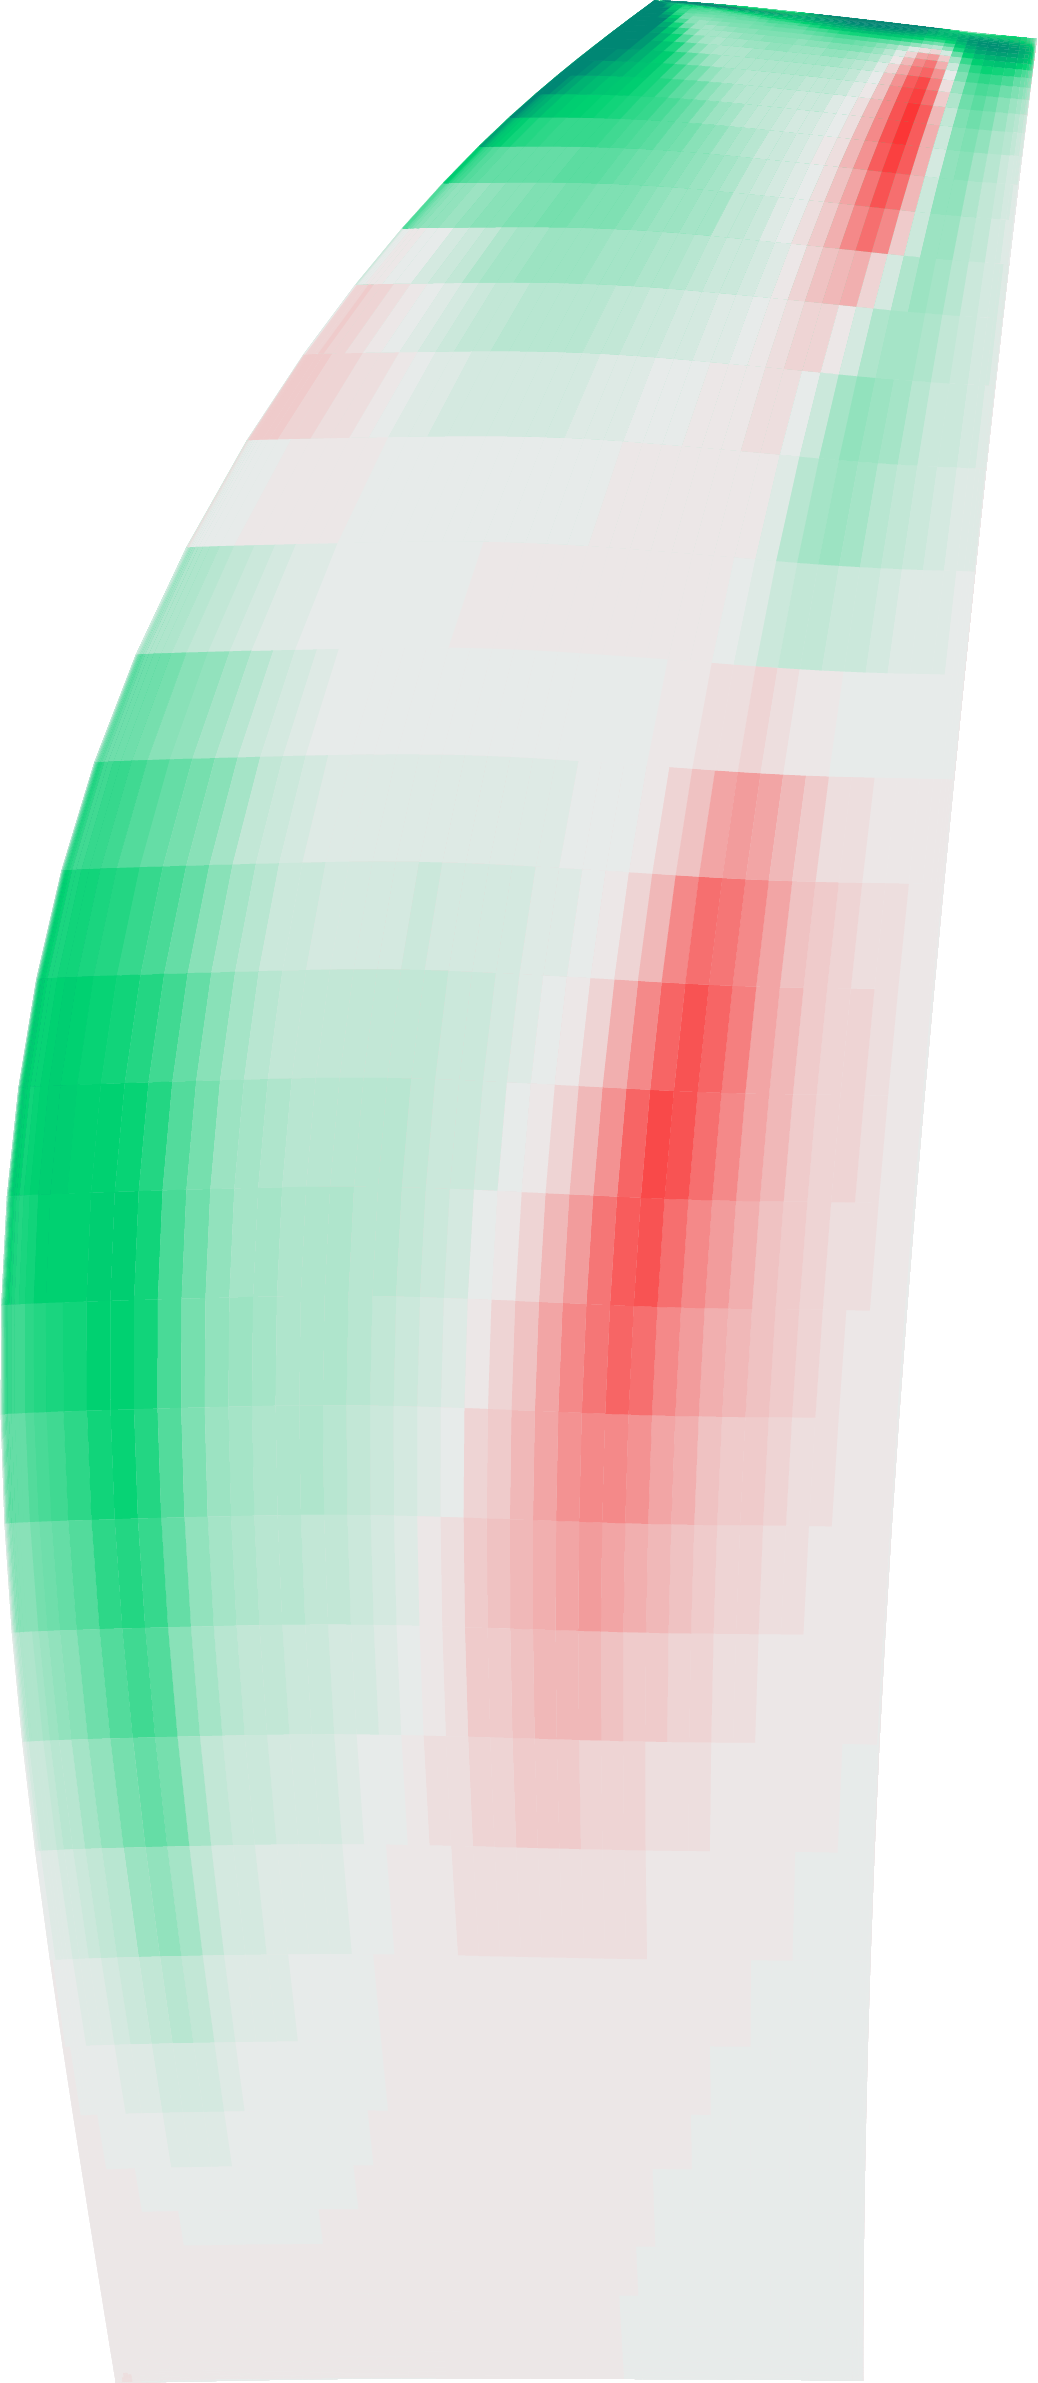
\includegraphics[width=0.12\textwidth]{DREAM_HS_HBT_N3_AEL_H1M2FD-1_roe3_sa_local_damping_SS.png}
   & 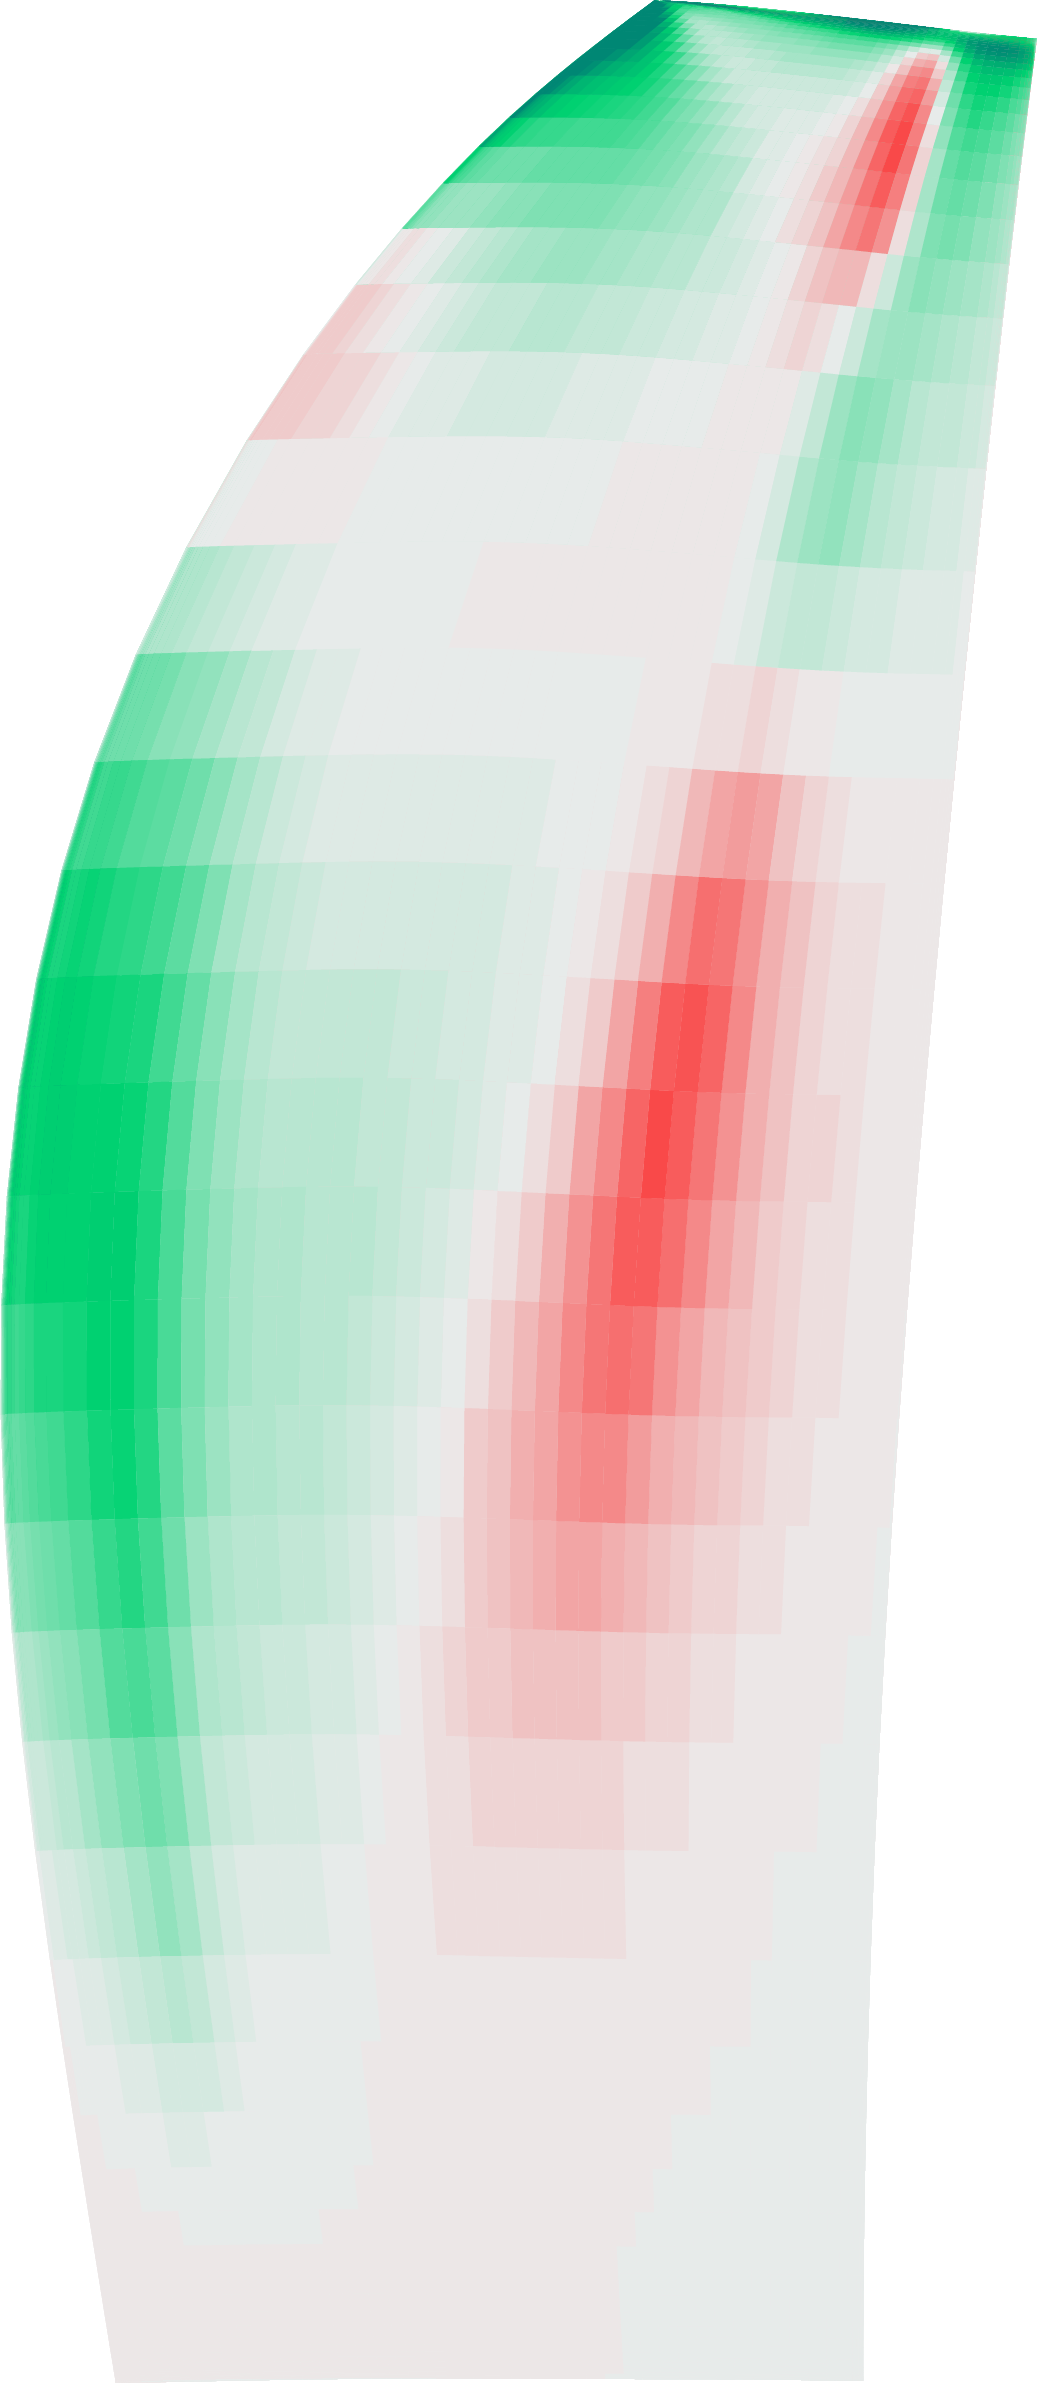
\includegraphics[width=0.12\textwidth]{DREAM_HS_HBT_N4_AEL_H1M2FD-1_roe3_sa_local_damping_SS.png}
   & 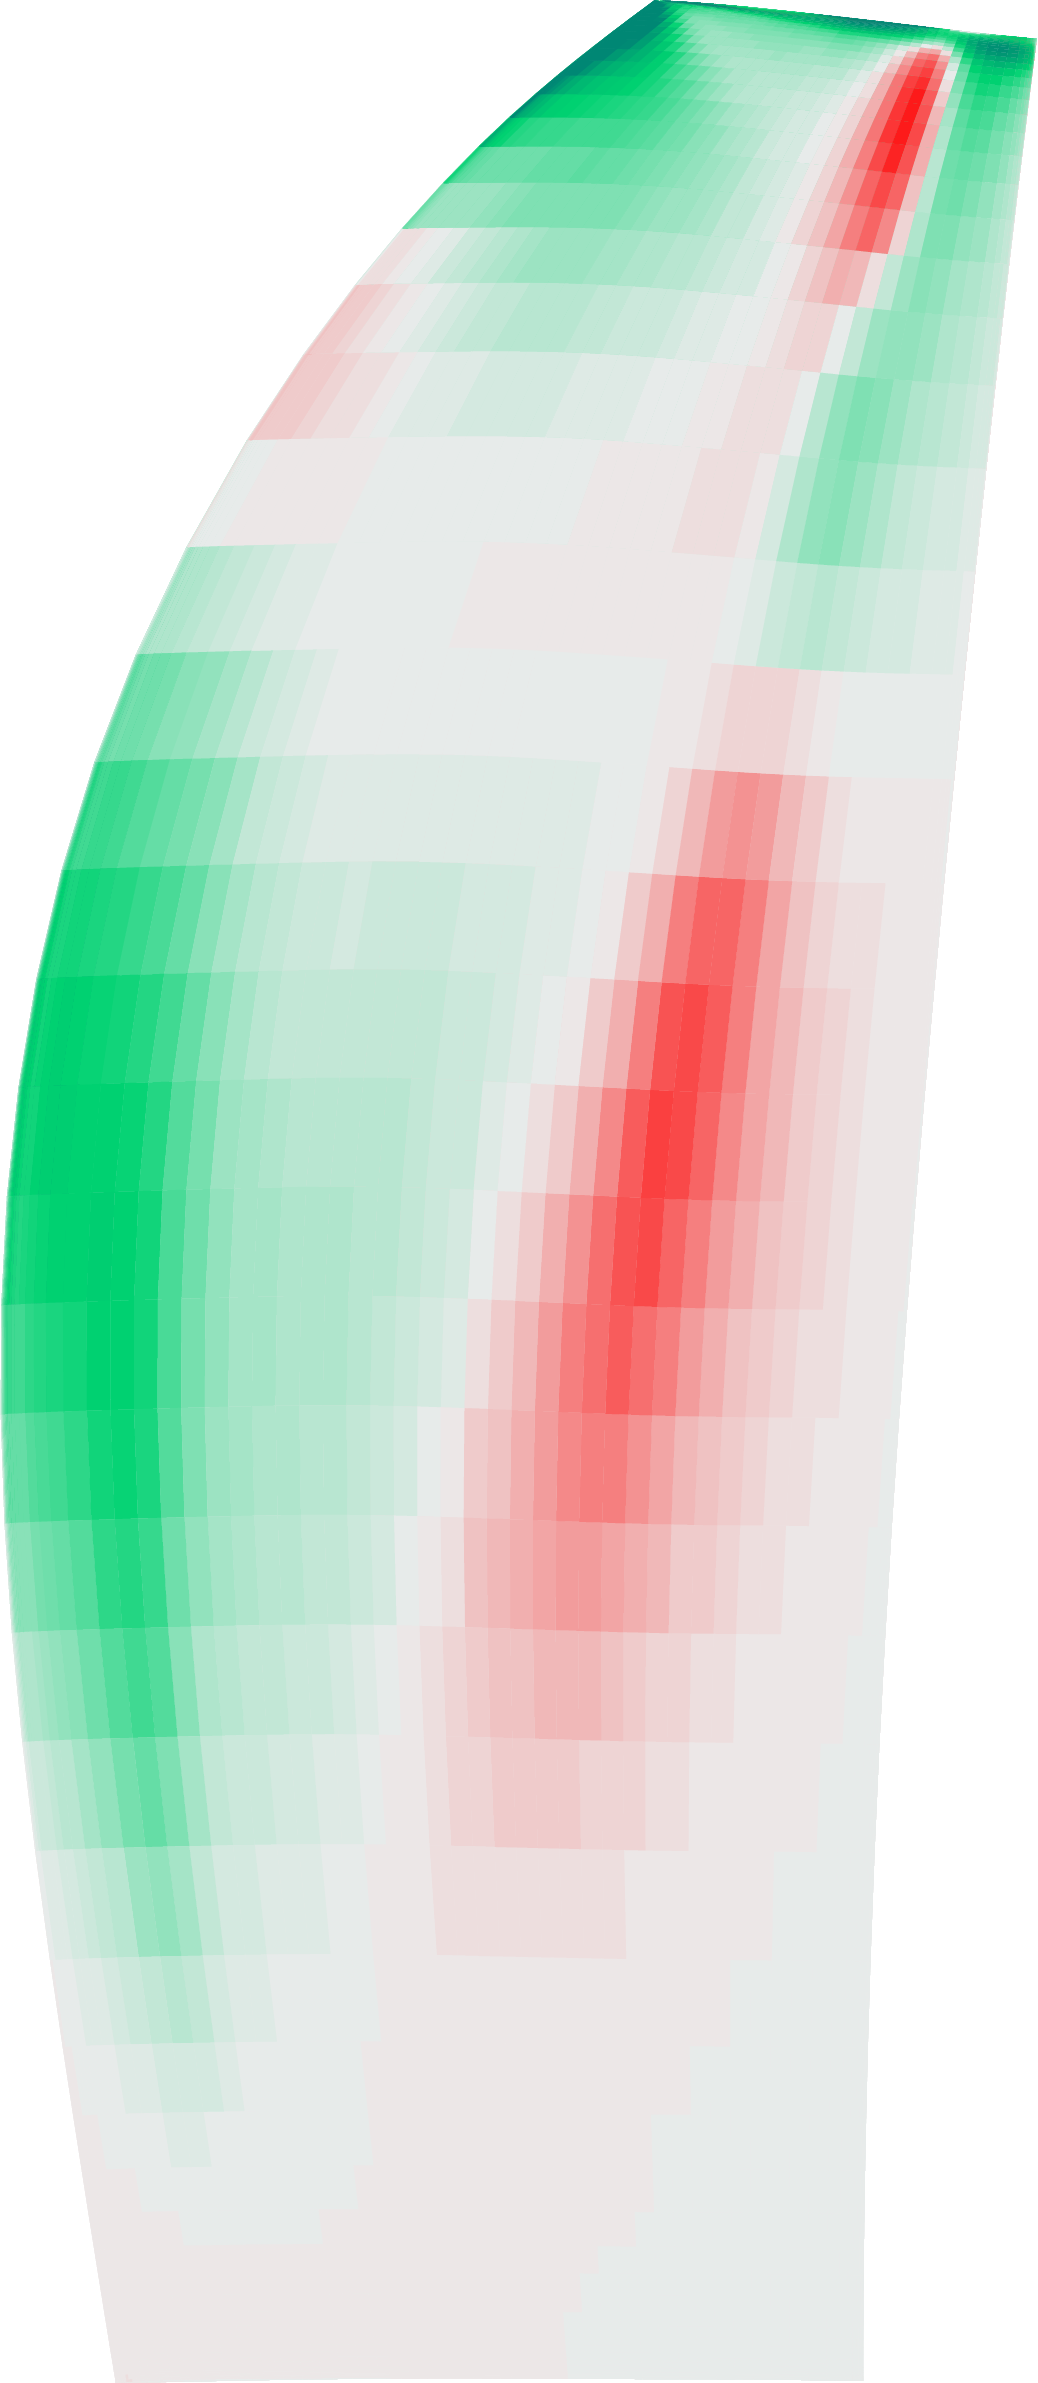
\includegraphics[width=0.12\textwidth]{DREAM_HS_HBT_N5_AEL_H1M2FD-1_roe3_sa_local_damping_SS.png} \\
   \rotatebox{90}{\quad\quad\quad pressure side} 
   & 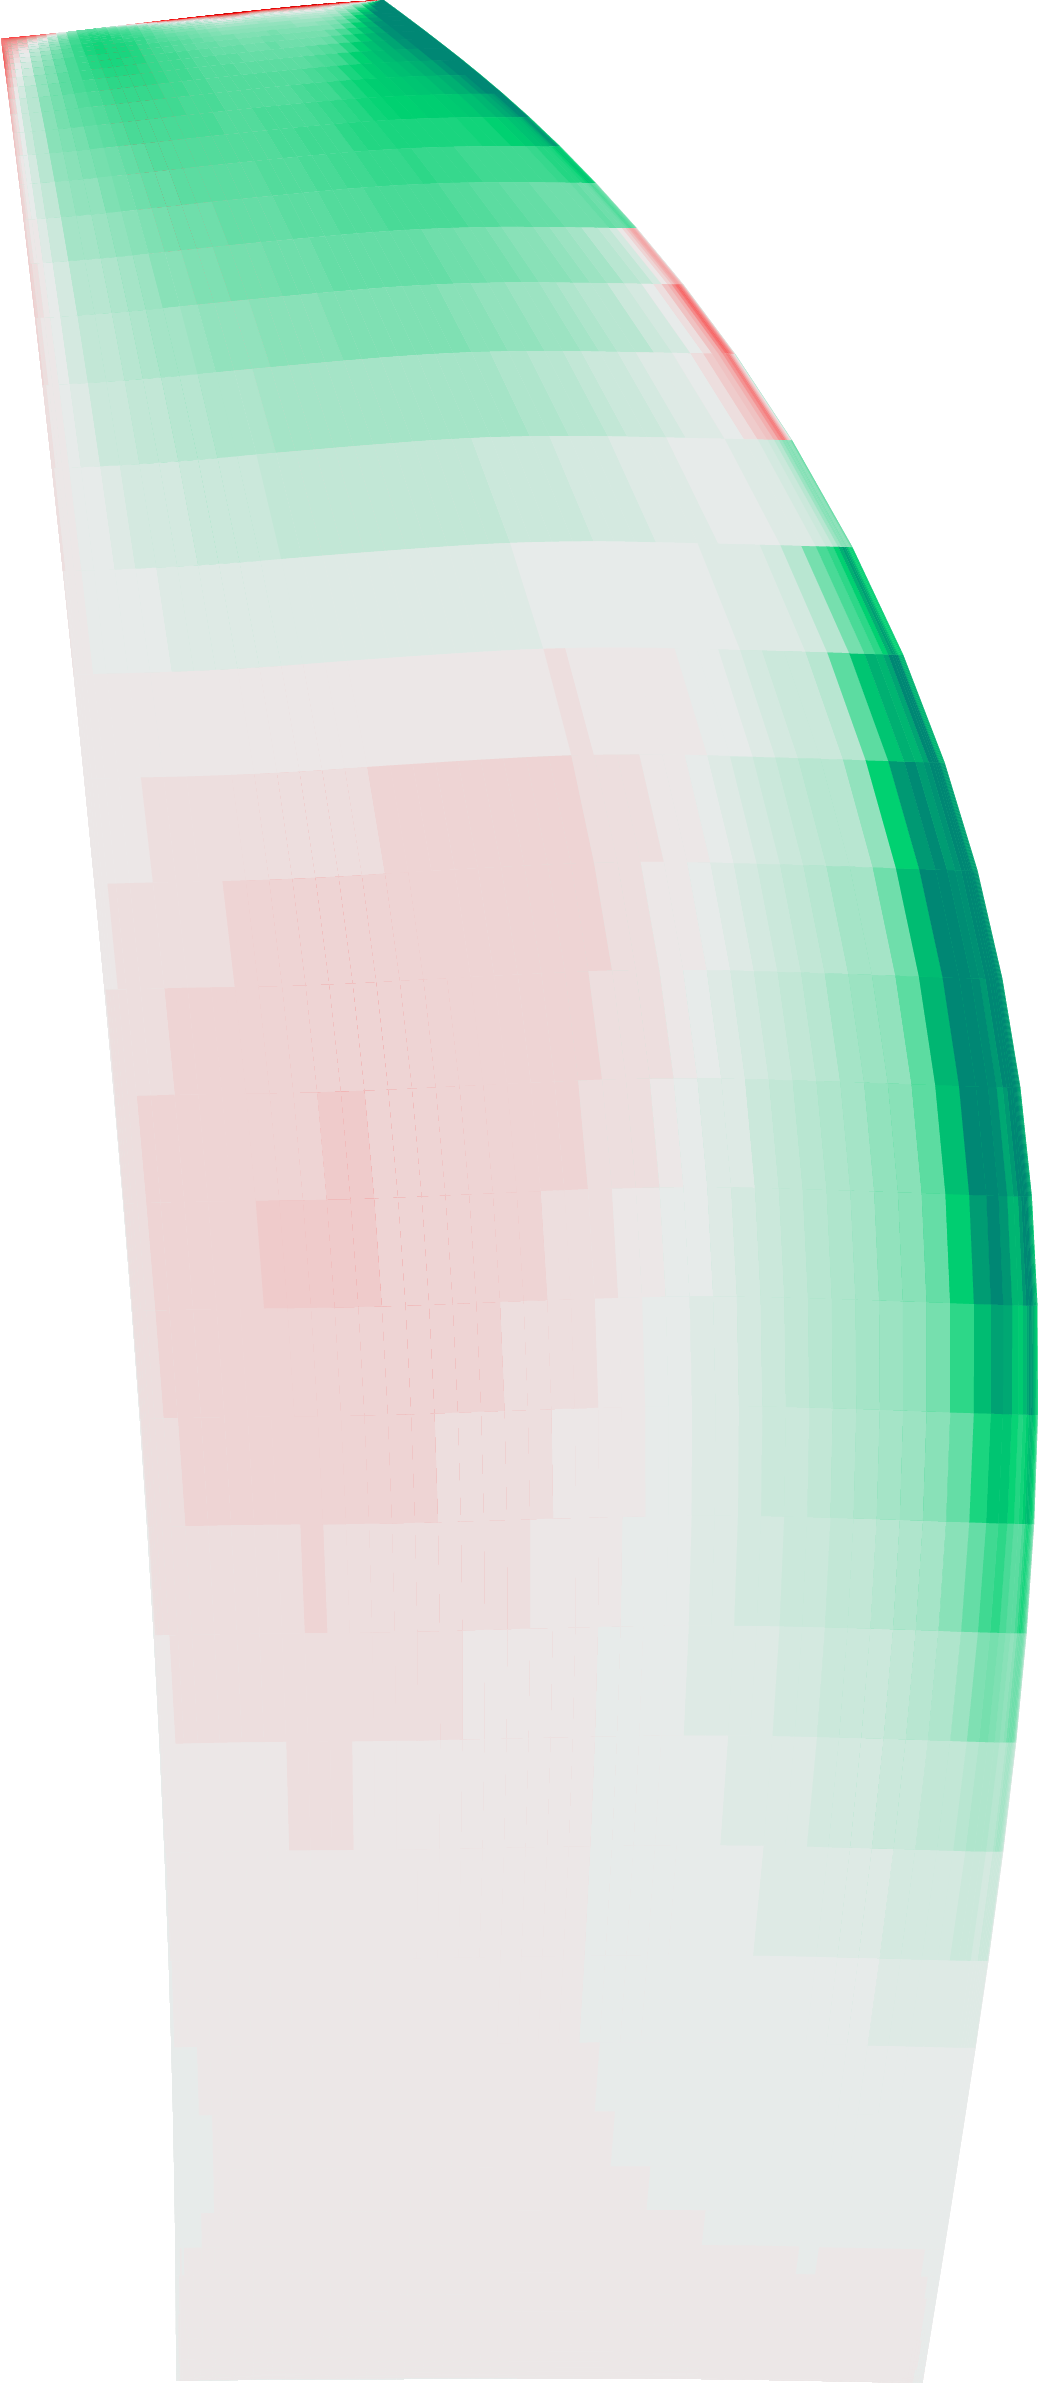
\includegraphics[width=0.12\textwidth]{DREAM_HS_HBT_N2_AEL_H1M2FD-1_roe3_sa_local_damping_PS.png}
   & 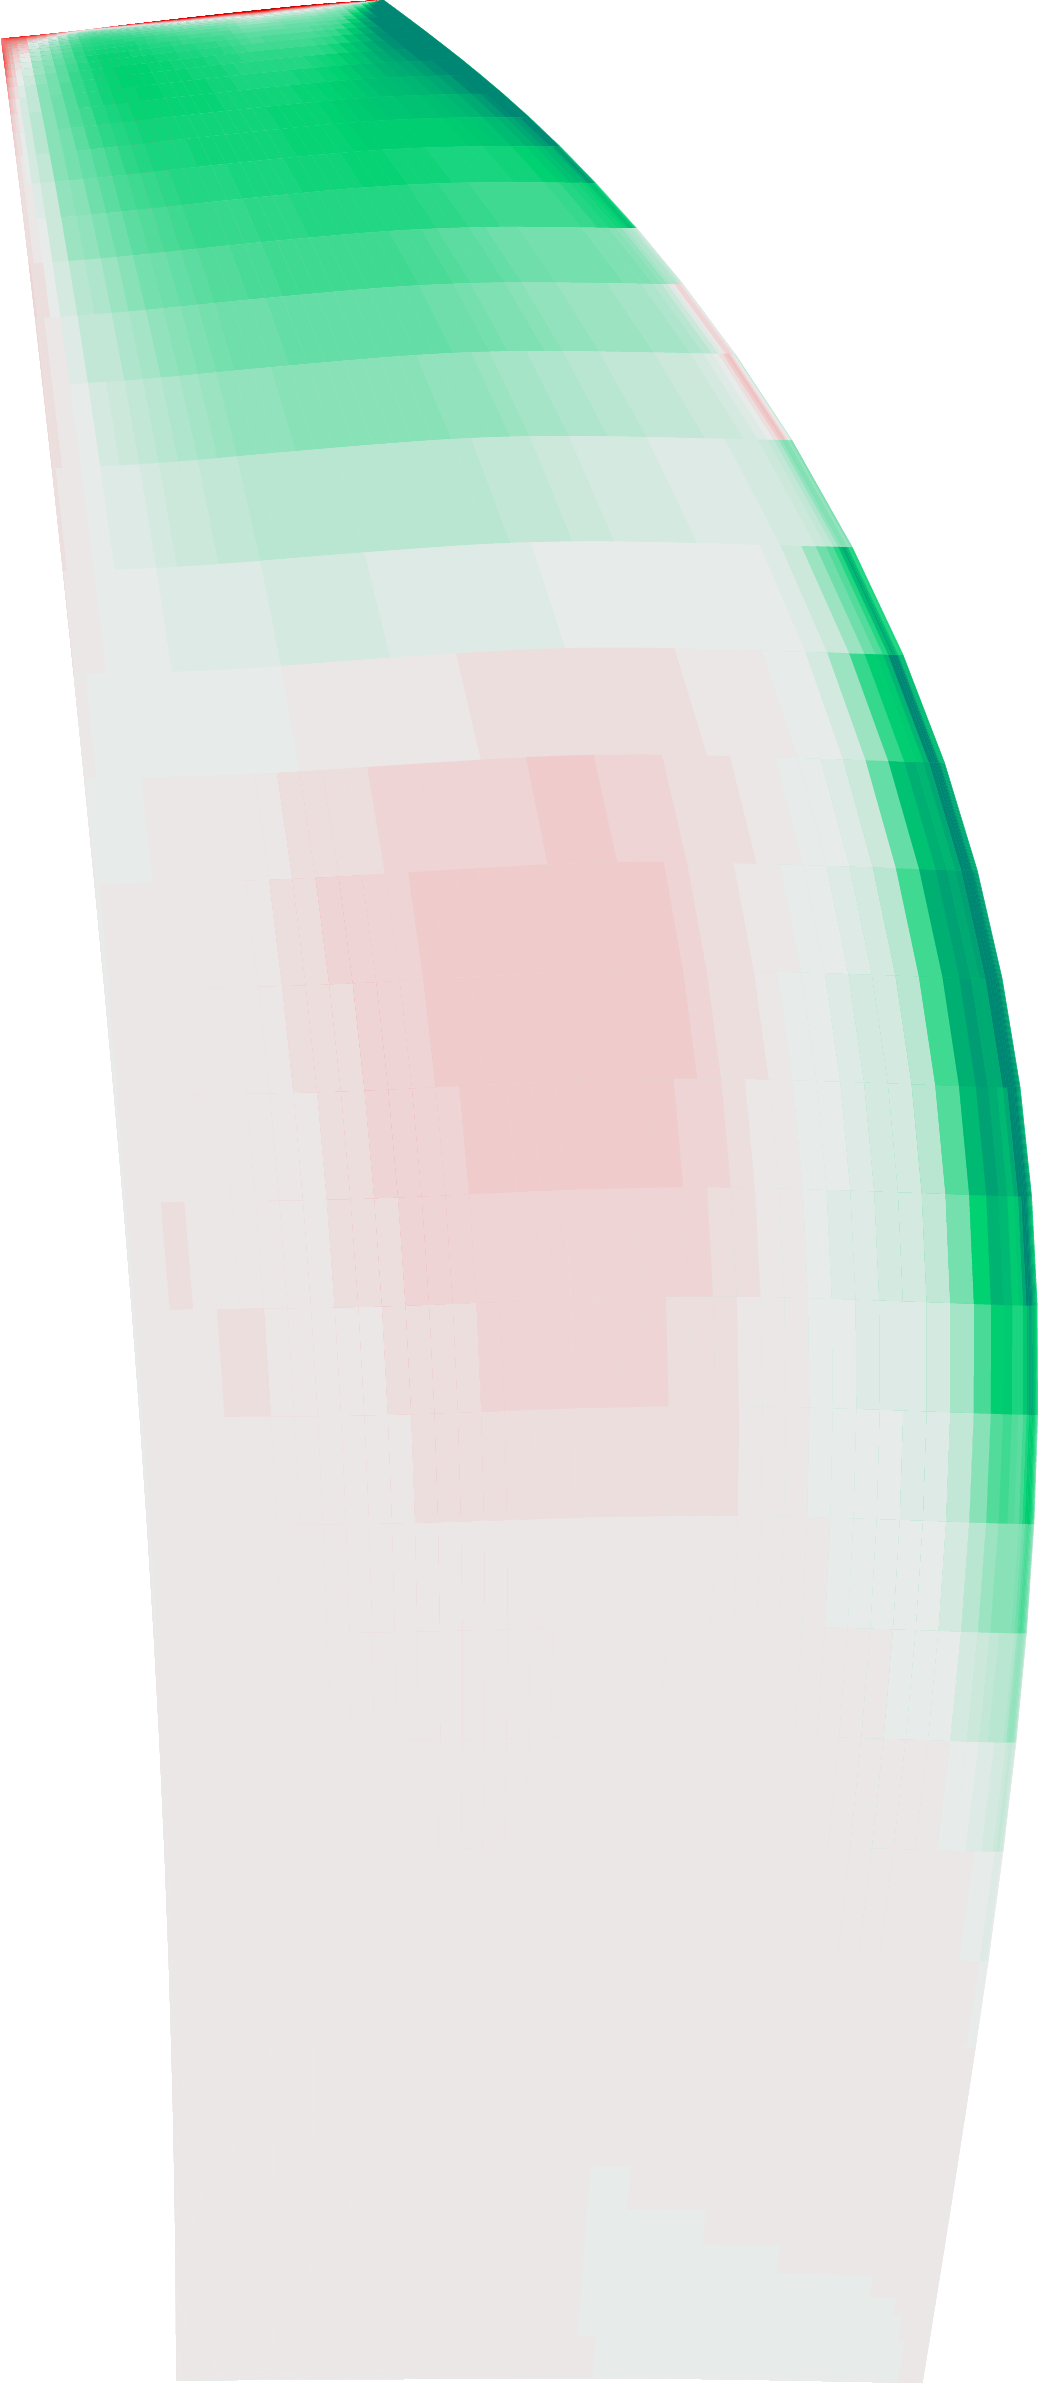
\includegraphics[width=0.12\textwidth]{DREAM_HS_HBT_N3_AEL_H1M2FD-1_roe3_sa_local_damping_PS.png}
   & 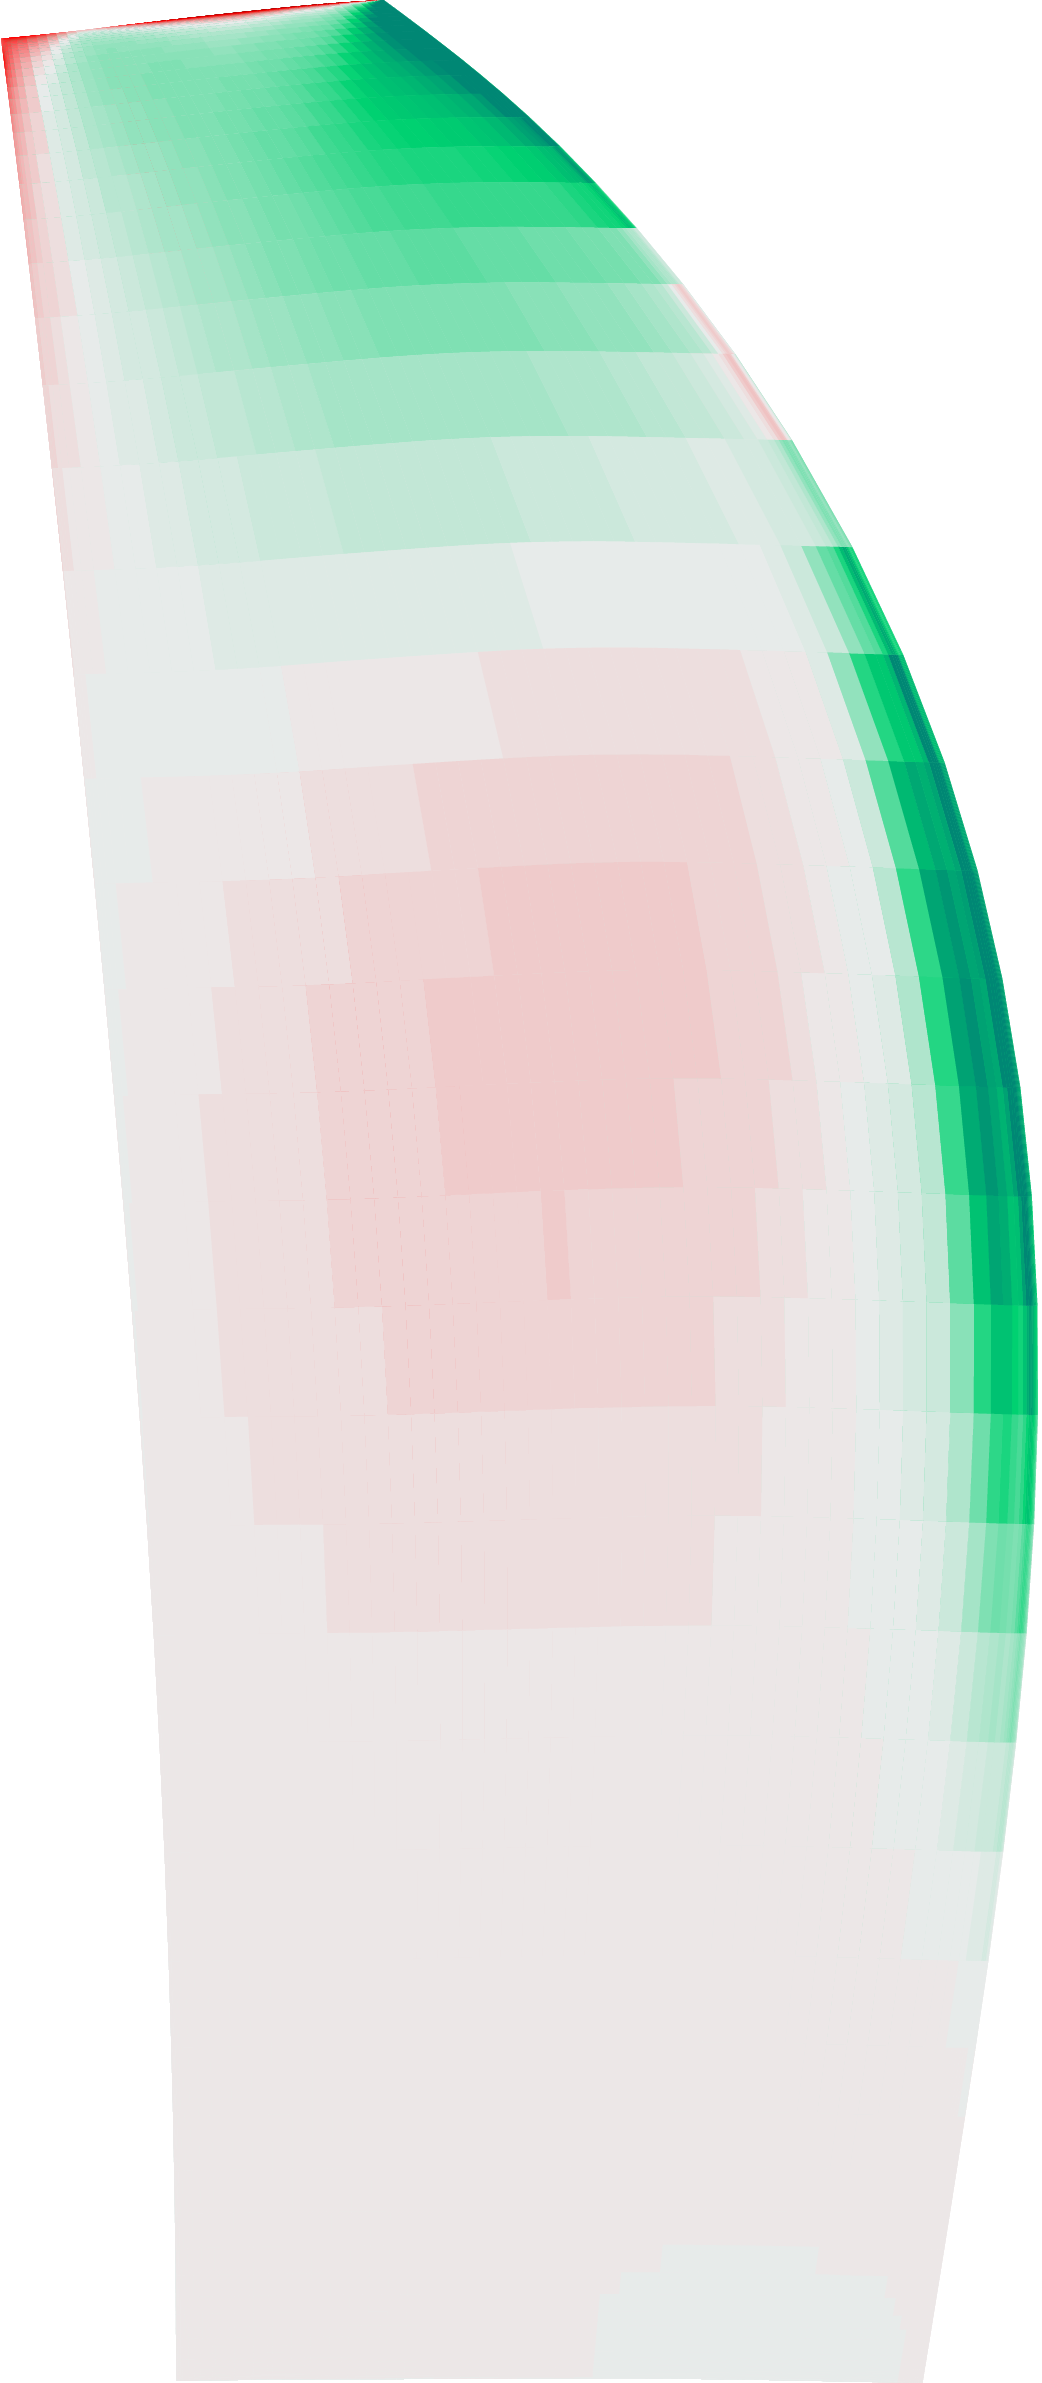
\includegraphics[width=0.12\textwidth]{DREAM_HS_HBT_N4_AEL_H1M2FD-1_roe3_sa_local_damping_PS.png}
   & 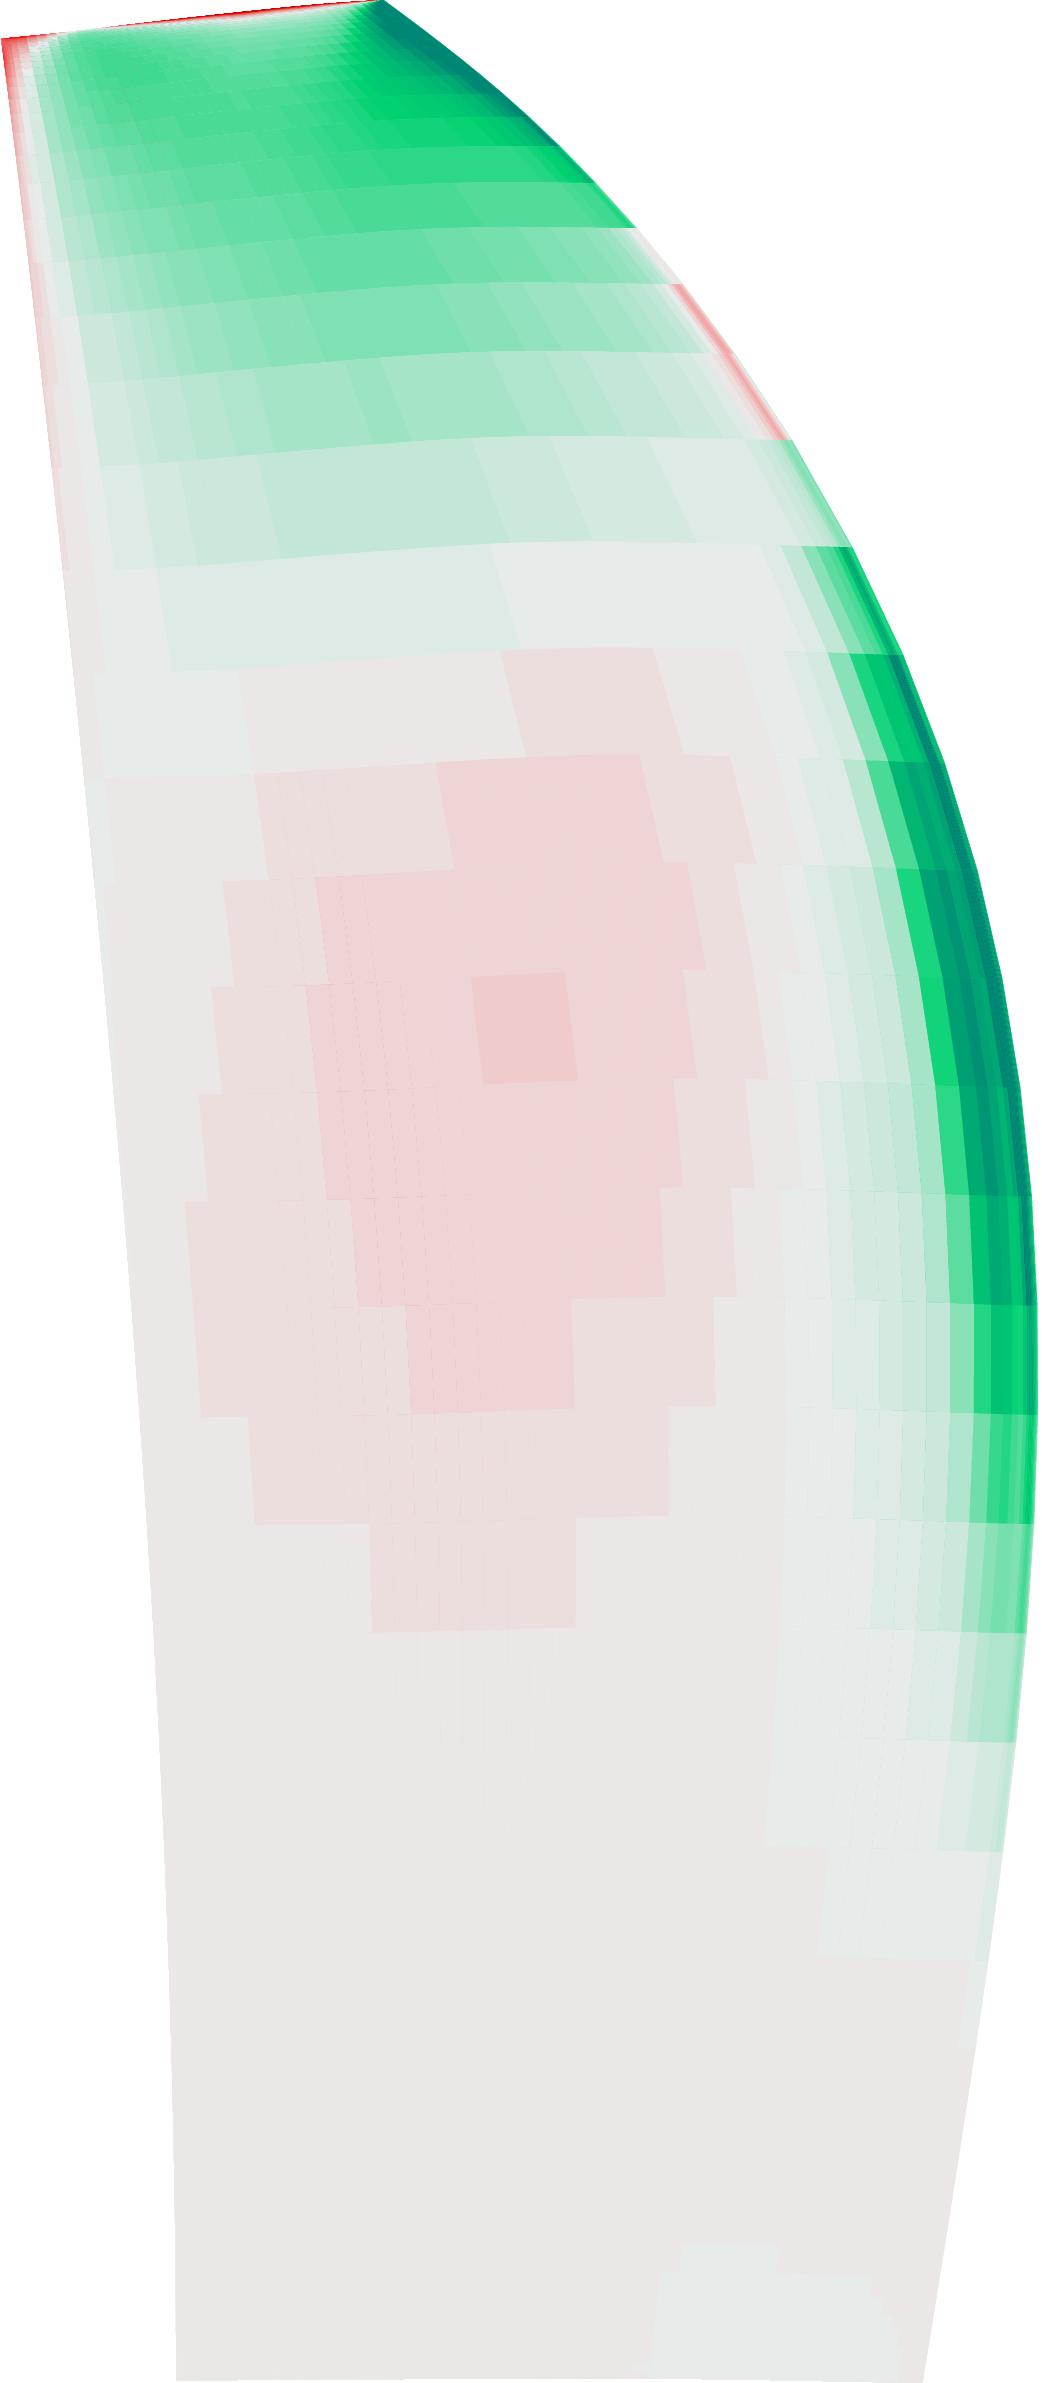
\includegraphics[width=0.12\textwidth]{DREAM_HS_HBT_N5_AEL_H1M2FD-1_roe3_sa_local_damping_PS.png} \\
   \bottomrule
   \multicolumn{1}{c}{}& \\
   \multicolumn{1}{c}{} & \multicolumn{4}{c}{
        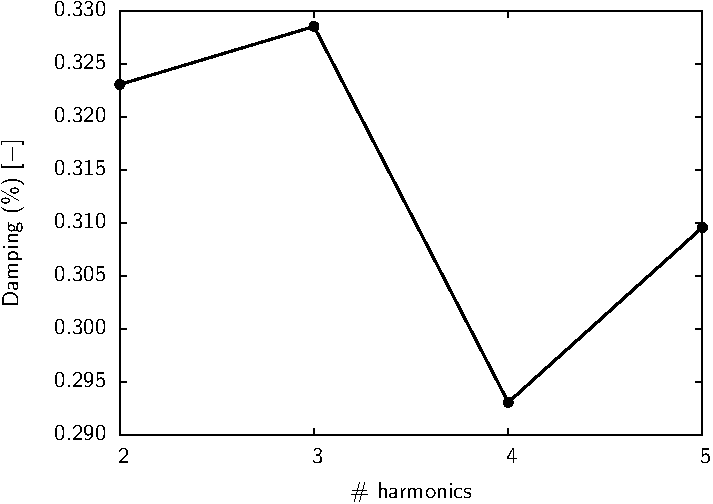
\includegraphics[width=0.45\textwidth]{DREAM_HS_COMVERGENCE_DAMPING.pdf}} \\
 \end{tabular}
 \caption{High-speed isolated configuration: convergence of local excitation and damping.}
 \label{fig:dream_hs_ael_convergence_damping}
\end{figure}
Raising the number of harmonics of the rear rotor blade passing frequency
changes the damping by at-most 10\% but the contours
of the local excitation are kept unchanged. Only small differences
are observed, that integrated produces the 10\%
observed on the damping value. Further investigation of the
convergence for the choice of frequencies are needed, but
this has not been done on this work.
Therefore, we will consider the $N=5$ aeroelastic
computations for the following.

\paragraph{Influence of the spatial discretization}
\label{sub:dream_hs_spatial_discretization}

To assess the different spatial scheme for this high-speed
CROR configuration, the same exercise as done in 
Sec.~\ref{sub:dream_ls_spatial_discretization} is made below.
Four schemes are evaluated based 
on the convergence of the computation
and of the integrated 
results (similarity coefficients).
For the \citet{Jameson1981} scheme, the artificial viscosities
are chosen as follow: $\kappa_2 = 1.0$ as the configuration is likely to 
see shocks and $\kappa_4 = 0.016$. We will see that the computation converges
with this low $\kappa_4$ coefficient. Therefore, only this coefficient
will be tested.

The convergence of the computations using the four spatial schemes
is shown in Figure~\ref{fig:DREAM_HS_RESIDUALS_PPT}. The convergence is good
for all the spatial schemes. In fact, more than five order of magnitude
is lost on the residuals.
\begin{figure}[htp]
  \centering
  \includegraphics*[width=0.50\textwidth]{SPACE_SCHEME_DIFF_HS_RESIDUALS.pdf}
  \caption{High-speed isolated configuration: convergence 
  of steady computations using different spatial schemes.}
  \label{fig:DREAM_HS_RESIDUALS_PPT}
\end{figure}

The values of the similarity coefficients obtained with
all the spatial schemes is reported in 
Figure~\ref{fig:dream_hs_space_scheme_coeff}. Arbitrarily, the values are
given as a ratio over the Roe~2 values. The first-order
upwind scheme (Roe~1) give similarity coefficients that are
several percent lower than the Roe~2 value. The other schemes
give results that are less than 1\% close, therefore and for
consistence with the approach retained for the LS configuration
the Roe~2 scheme is chosen for the following results.
\begin{figure}[htp]
  \centering
  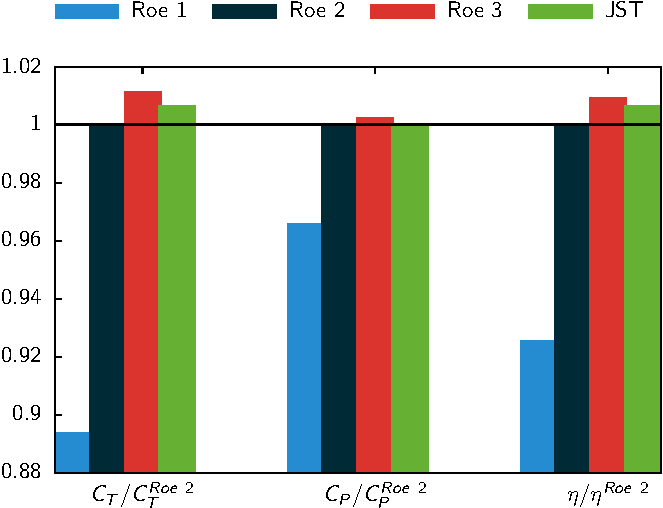
\includegraphics[width=.5\textwidth]{SPACE_SCHEME_DIFF_HS_COEFF.pdf}
  \caption{High-speed isolated configuration: convergence of 
  similarity coefficients using different spatial schemes.}
  \label{fig:dream_hs_space_scheme_coeff}
\end{figure}

